\documentclass[tikz,border=8pt]{standalone}
\usepackage{tikz}
\usetikzlibrary{arrows.meta,calc}

\definecolor{primary}{HTML}{143264}
\definecolor{secondary}{HTML}{8C281E}
\definecolor{tealcol}{HTML}{117A65}
\definecolor{orangecol}{HTML}{C77C02}
\definecolor{purplecol}{HTML}{6A3D9A}
\definecolor{greycol}{HTML}{505A64}

\begin{document}
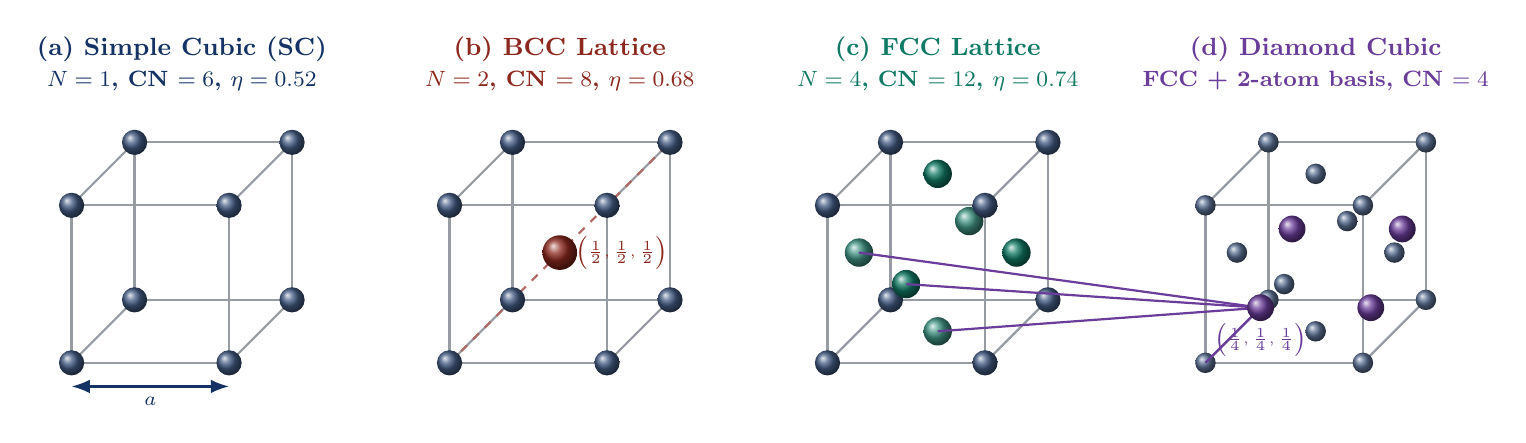
\begin{tikzpicture}[>=Latex]

  % Subfigure (a): Simple Cubic (SC)
  \begin{scope}[shift={(0,0)}]
    \node[align=center, font=\bfseries\small, text=primary] at (1.4, 3.8) {(a) Simple Cubic (SC)\\ \footnotesize $N=1$, CN $=6$, $\eta=0.52$};
    \draw[thick, greycol!60] (0,0) coordinate (O) -- (2,0) coordinate (A) -- (2,2) coordinate (B) -- (0,2) coordinate (C) -- cycle;
    \draw[thick, greycol!60] (0.8,0.8) coordinate (O') -- (2.8,0.8) coordinate (A') -- (2.8,2.8) coordinate (B') -- (0.8,2.8) coordinate (C') -- cycle;
    \draw[thick, greycol!60] (O) -- (O') (A) -- (A') (B) -- (B') (C) -- (C');
    \draw[<->, primary, thick] (0,-0.3) -- (2,-0.3) node[midway, below, font=\scriptsize] {$a$};
    \foreach \pt in {O,A,B,C,O',A',B',C'} {
      \shade[ball color=primary!80] (\pt) circle (0.16);
    }
  \end{scope}

  % Subfigure (b): Body-Centered Cubic (BCC)
  \begin{scope}[shift={(4.8,0)}]
    \node[align=center, font=\bfseries\small, text=secondary] at (1.4, 3.8) {(b) BCC Lattice\\ \footnotesize $N=2$, CN $=8$, $\eta=0.68$};
    \draw[thick, greycol!60] (0,0) coordinate (O) -- (2,0) coordinate (A) -- (2,2) coordinate (B) -- (0,2) coordinate (C) -- cycle;
    \draw[thick, greycol!60] (0.8,0.8) coordinate (O') -- (2.8,0.8) coordinate (A') -- (2.8,2.8) coordinate (B') -- (0.8,2.8) coordinate (C') -- cycle;
    \draw[thick, greycol!60] (O) -- (O') (A) -- (A') (B) -- (B') (C) -- (C');
    \draw[dashed, secondary!70, thick] (O) -- (B');
    \coordinate (BC) at (1.4, 1.4);
    \shade[ball color=secondary] (BC) circle (0.22);
    \foreach \pt in {O,A,B,C,O',A',B',C'} {
      \shade[ball color=primary!80] (\pt) circle (0.16);
    }
    \node[right=2pt, font=\tiny\bfseries, secondary] at (BC) {$\left(\frac{1}{2},\frac{1}{2},\frac{1}{2}\right)$};
  \end{scope}

  % Subfigure (c): Face-Centered Cubic (FCC)
  \begin{scope}[shift={(9.6,0)}]
    \node[align=center, font=\bfseries\small, text=tealcol] at (1.4, 3.8) {(c) FCC Lattice\\ \footnotesize $N=4$, CN $=12$, $\eta=0.74$};
    \draw[thick, greycol!60] (0,0) coordinate (O) -- (2,0) coordinate (A) -- (2,2) coordinate (B) -- (0,2) coordinate (C) -- cycle;
    \draw[thick, greycol!60] (0.8,0.8) coordinate (O') -- (2.8,0.8) coordinate (A') -- (2.8,2.8) coordinate (B') -- (0.8,2.8) coordinate (C') -- cycle;
    \draw[thick, greycol!60] (O) -- (O') (A) -- (A') (B) -- (B') (C) -- (C');
    \coordinate (Ffront) at (1,1);
    \coordinate (Fback) at (1.8, 1.8);
    \coordinate (Fbot) at (1.4, 0.4);
    \coordinate (Ftop) at (1.4, 2.4);
    \coordinate (Fleft) at (0.4, 1.4);
    \coordinate (Fright) at (2.4, 1.4);
    \shade[ball color=tealcol!80] (Fback) circle (0.18);
    \shade[ball color=tealcol!80] (Fleft) circle (0.18);
    \shade[ball color=tealcol!80] (Fbot) circle (0.18);
    \foreach \pt in {O,A,B,C,O',A',B',C'} {
      \shade[ball color=primary!80] (\pt) circle (0.16);
    }
    \shade[ball color=tealcol] (Ffront) circle (0.18);
    \shade[ball color=tealcol] (Ftop) circle (0.18);
    \shade[ball color=tealcol] (Fright) circle (0.18);
  \end{scope}

  % Subfigure (d): Diamond Cubic Basis
  \begin{scope}[shift={(14.4,0)}]
    \node[align=center, font=\bfseries\small, text=purplecol] at (1.4, 3.8) {(d) Diamond Cubic\\ \footnotesize FCC + 2-atom basis, CN $=4$};
    \draw[thick, greycol!60] (0,0) coordinate (O) -- (2,0) coordinate (A) -- (2,2) coordinate (B) -- (0,2) coordinate (C) -- cycle;
    \draw[thick, greycol!60] (0.8,0.8) coordinate (O') -- (2.8,0.8) coordinate (A') -- (2.8,2.8) coordinate (B') -- (0.8,2.8) coordinate (C') -- cycle;
    \draw[thick, greycol!60] (O) -- (O') (A) -- (A') (B) -- (B') (C) -- (C');
    \foreach \pt in {O,A,B,C,O',A',B',C'} {
      \shade[ball color=primary!70] (\pt) circle (0.13);
    }
    \foreach \fc in {(1,1), (1.8,1.8), (1.4,0.4), (1.4,2.4), (0.4,1.4), (2.4,1.4)} {
      \shade[ball color=primary!70] \fc circle (0.13);
    }
    \coordinate (T1) at (0.7, 0.7);
    \coordinate (T2) at (2.1, 0.7);
    \coordinate (T3) at (1.1, 1.7);
    \coordinate (T4) at (2.5, 1.7);
    \draw[thick, purplecol] (O) -- (T1);
    \draw[thick, purplecol] (Ffront) -- (T1);
    \draw[thick, purplecol] (Fbot) -- (T1);
    \draw[thick, purplecol] (Fleft) -- (T1);
    \shade[ball color=purplecol] (T1) circle (0.17);
    \shade[ball color=purplecol] (T2) circle (0.17);
    \shade[ball color=purplecol] (T3) circle (0.17);
    \shade[ball color=purplecol] (T4) circle (0.17);
    \node[below=2pt, font=\tiny\bfseries, purplecol] at (T1) {$\left(\frac{1}{4},\frac{1}{4},\frac{1}{4}\right)$};
  \end{scope}

\end{tikzpicture}
\end{document}
